\section[Background and motivation]{Background and motivation}
In mid 1993 Ihaka and Gentleman published initial efforts on the computing
language and programming environment R on the s-news mailing list. Ambitions for
this project aimed to develop an S-like language but without inheriting memory
and performance issues. The source code of R was finally released in 1995 and
development has since evolved under the umbrella of the R Development Core Team
since mid 1997 \citep{RDCT2001, RDCT2010, Ihaka_Gentlemen_1993}.
R does not include an advanced cross-platform GUI as known from other
statistical software packages. However, R includes tools for building GUIs
mainly based on Tlc/Tk \citep{Dalgaard2001, Dalgaard2002}. Since then a
plethora of R GUIs have emerged (see \url{http://www.sciviews.org/_rgui/} for a
comprehensive list). In 2005 John Fox released version 1.0 of R Commander which
can be considered a milestone in R GUI development; this was the first GUI
implementation which was able to deliver the experience of statistical tests,
plots and data manipulation easily accessible for R novices as well as advanced
users. However, John Fox stated that R Commander's target was to provide
functionality for basic-statistical courses though functionality increased over
time beyond this \citep{Fox2005}. In November 2002 Thomas Friedrichsmeier
started the RKWard open-source software project with the goal to create an
implementation of an R GUI based on KDE and Qt technologies.

The scope of RKWard is deliberately broad, targeting both R novices and experts.
Regarding the first group, the aim is to allow any person with knowledge on
statistical procedures to start using RKWard for their everyday work,
immediately, without having to learn anything about the R programming language,
first. At the same time RKWard tries to support users who want to learn and
exploit the full flexibility of the R language for automating or customizing
analyses. At the other end of the learning curve, RKWard provides advanced IDE
features to R experts to assist in the development of R scripts. Yet, the idea
is that R experts, too will benefit from the availability task-oriented GUI
dialogs from time to time, such as when exploring an unfamiliar type of analysis
or by allowing to implement routinely performed tasks as a GUI element. In
addition, many features, such as the integrated data editor, or the plot preview
feature will be useful to R novices and R experts alike in their everyday work
(see section \ref{Default Graphical User Interface Elements}).

%% TODO: TF: I have edited this section (and the following) a bit more. Please take a look.
RKWard provides a high level of transparency about the steps that are needed to
perform any supported task in R, in order to make it easy for the user to see
complete code for all GUI actions. In doing so RKWard accepts relatively verbose
generated code, deliberately. In particular, RKWard limits itself to generate R
code from GUI settings. It avoids wrapping complex sequences of data
manipulation or analysis into custom high-level R functions. The task of
providing high-level functions is logically independent of the development the
GUI frontend, and should best be solved in dedicated R packages, where needed.
This approach allows to make better use of the modular design of R, avoids
locking in users to a specific GUI solution, and allows them more options for
customizing generated code patterns.

While RKWard tries to support users wishing to learn R, it is specifically not
designed as a teaching tool (such as \pkg{Rcmdr} or \pkg{TeachingDemos}), but as
a productive tool. Dialogs for statistical procedures in RKWard do not
necessarily show a 1:1 correspondence to the underlying steps in R, but are
rather oriented at statistical tasks. Furthermore, RKWard does not impose
artificial limitations on how users can work with the application. For example,
the user is not limited to using only one \code{data.frame} or one model at a
time, in RKWard. RKWard is designed to allow users to create custom GUI dialogs
easily (see sections \ref{technical_plugins} and \ref{example_plugins}).

%% TODO: TF: I've removed the reference to ``Beta''-status. It's just an arbitrary estimate without a real definition, anyway.
%% Please take a look at the wording I have added, instead.
RKWard is licensed under the terms of the GNU General Public License Version 2
or later. This means the RKWard code itself is GPL v 2 or 3 but effectively
distributable only under GPL v 2 due to R code. Some documentation templates are
GFDL licensed. While the project remains in constant development, a growing
number of users employs RKWard in productive scenarios. The source code,
selected binaries and documentation is hosted at SourceForge
(http://sourceforge.net/). Milestones of the RKWards development are
demonstrated in Figure~\ref{fig:timeline}.

\begin{figure}[htp]
 \centering
 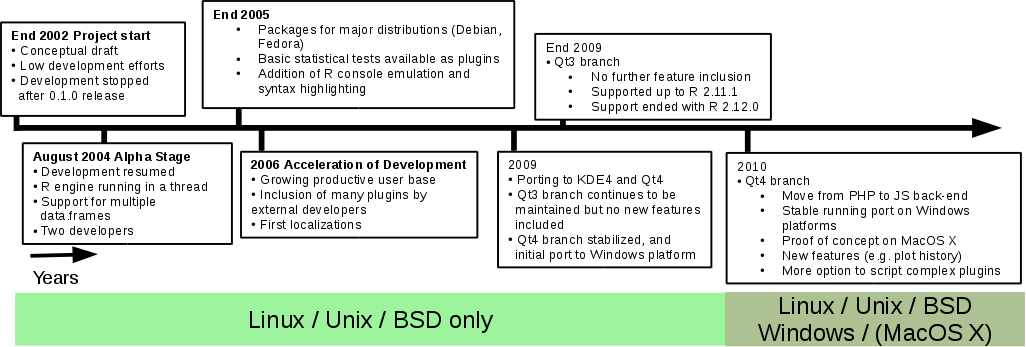
\includegraphics{../figures/timeline.png}
 \caption{Timeline of important development milestones and changes in RKWard.
          Time is presented on an arbitrary scale.}
 \label{fig:timeline}
\end{figure}

In this paper we will first give an overview over the main GUI elements and
features of RKWard. Next some technical aspects of the implementation will be
dicussed, comparing them briefly to competing GUI solutions, where appropriate.
The paper concludes with an example of a simple RKWard session. Additionally,
we show an example for creating a simple plugin extension to RKWard.
